\chapter{Testing}

\cjorge{VOY REVISANDO POR AQUÍ...}

We can now proceed into testing both scenarios and see how they perform when traffic is injected into the network. 

\section{Port Slicing}
For the tests regarding this type of slicing, we have not used real traffic as we just wanted to see if the slicing itself works, instead we have used a tool called Iperf. It allows us to generate either TCP or UDP traffic and it reports back with the bandwidth of the connection. The basic usage of Iperf goes as follows:
\begin{enumerate}
    \item On the end point, call Iperf to listen to a port.
    \begin{lstlisting}
    iperf -s -p <TCP_port_number>
    \end{lstlisting}
    
    \item Now, on a different host, send traffic to the end point.
    \begin{lstlisting}
    iperf -c <ip_address_endpoint> -p <TCP_port_number> -i 1
    \end{lstlisting}
\end{enumerate}

By default, Iperf sends a stream of small TCP packets for 10 seconds. To have a little more granularity, we add the switch \textit{-i 1}. This way we can see the bandwidth of the connection each second, instead of the average of a 10 seconds transmission.

Essentially, by looking at Iperf's bandwidth report, we can tell if the stream of packets is taking the slow or the fast path of the network. This is exactly what we have done, and by looking at Figures \ref{fig:iperf_port_9999} and \ref{fig:iperf_port_8000} we can confirm that the slicing is working as intended:
\begin{itemize}
    \item When the TCP connection is on port 9999, the bandwidth reported is \SIrange[per-mode=symbol]{7}{17}{\mega\bit\per\second}, which means the packets are taking the fast path. 
    \item Likewise, if the port is different from 9999, e.g, port 8000, the packets take the slow route and we see a bandwidth of \SIrange[per-mode=symbol]{1}{3}{\mega\bit\per\second}.
\end{itemize}

\begin{figure}
  \centering
  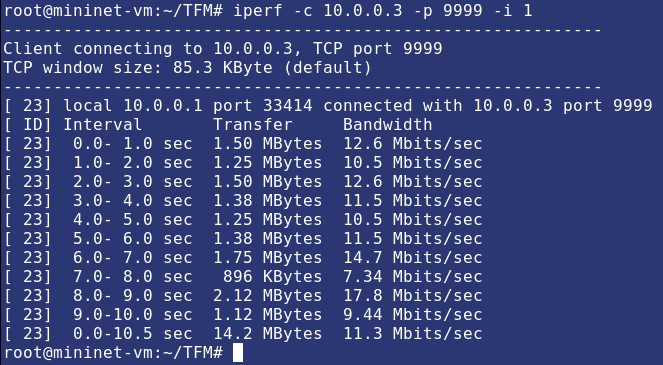
\includegraphics[width=\linewidth]{imagenes/Testing/port_slicing_iperf_fast.png}
  \caption{Iperf's bandwidth report of a TCP connection to port 9999, from host 1 to host 3.}
  \label{fig:iperf_port_9999}
\end{figure}

\begin{figure}
  \centering
  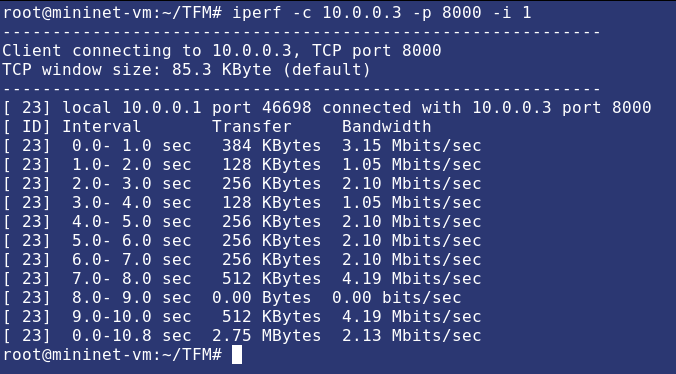
\includegraphics[width=\linewidth]{imagenes/Testing/port_slicing_iperf_slow.png}
  \caption{Iperf's bandwidth report of a TCP connection to port 8000, from host 1 to host 3.}
  \label{fig:iperf_port_8000}
\end{figure}

\subsection{Analysis of the Results}
While the bandwidth measurements are not entirely accurate, the margin between the tests is clear enough to warrant the correct slicing implementation, i.e. the packets take the intended path.

\cjorge{Yo cambiaría un poco el enfoque. VLAN usa port slicing usando el concepto de puerto de switch, no puerto de TCP/UDP. Así que diría que hace algo similar y por tanto el concepto no es nuevo. Pero igual, igual, no es.}

As it has been mentioned before, this type of network slicing is nothing new. Port based slicing is exactly what VLANs do in traditional networks and, in fact, have been widely used for many years. Nevertheless, it is still important to prove that port based slicing is still possible in the new network paradigm of SDNs.

\section{IP Address Slicing}
\subsection{Preparation}
In this scenario, we have performed a more advanced and complex test involving external hosts. While Iperf would have sufficed, we have opted for a test that closer resembles a real production environment, illustrated by Figured \ref{fig:topology_LoRa}. The physical setup is shown in Figure \ref{fig:LoRa_setup}. The main elements for this test are:
\begin{itemize}
    \item \textbf{LoRa mote}. It will broadcast packets over air using the LoRa protocol.
    \item \textbf{LoRa gateway}. Responsible for capturing the LoRa packets transmitted over air and forwarding them \cjorge{to the LoRaWAN network and application servers through the virtual Mininet network, which publish the messages using MQTT. Y QUITARÍA LO QUE SIGUE EN ESTE PÁRRAFO.}to the MQTT client through the virtual Mininet network. 
    \item \textbf{MQTT client}. If everything works correctly, it should receive the packets originally sent by the LoRa mote. In addition, these packets should traverse the Mininet network through the slow path. 
\end{itemize}

\cjorge{En esta figura faltan los servidores de red y aplicación LoRaWAN...}

\begin{figure}
  \centering
  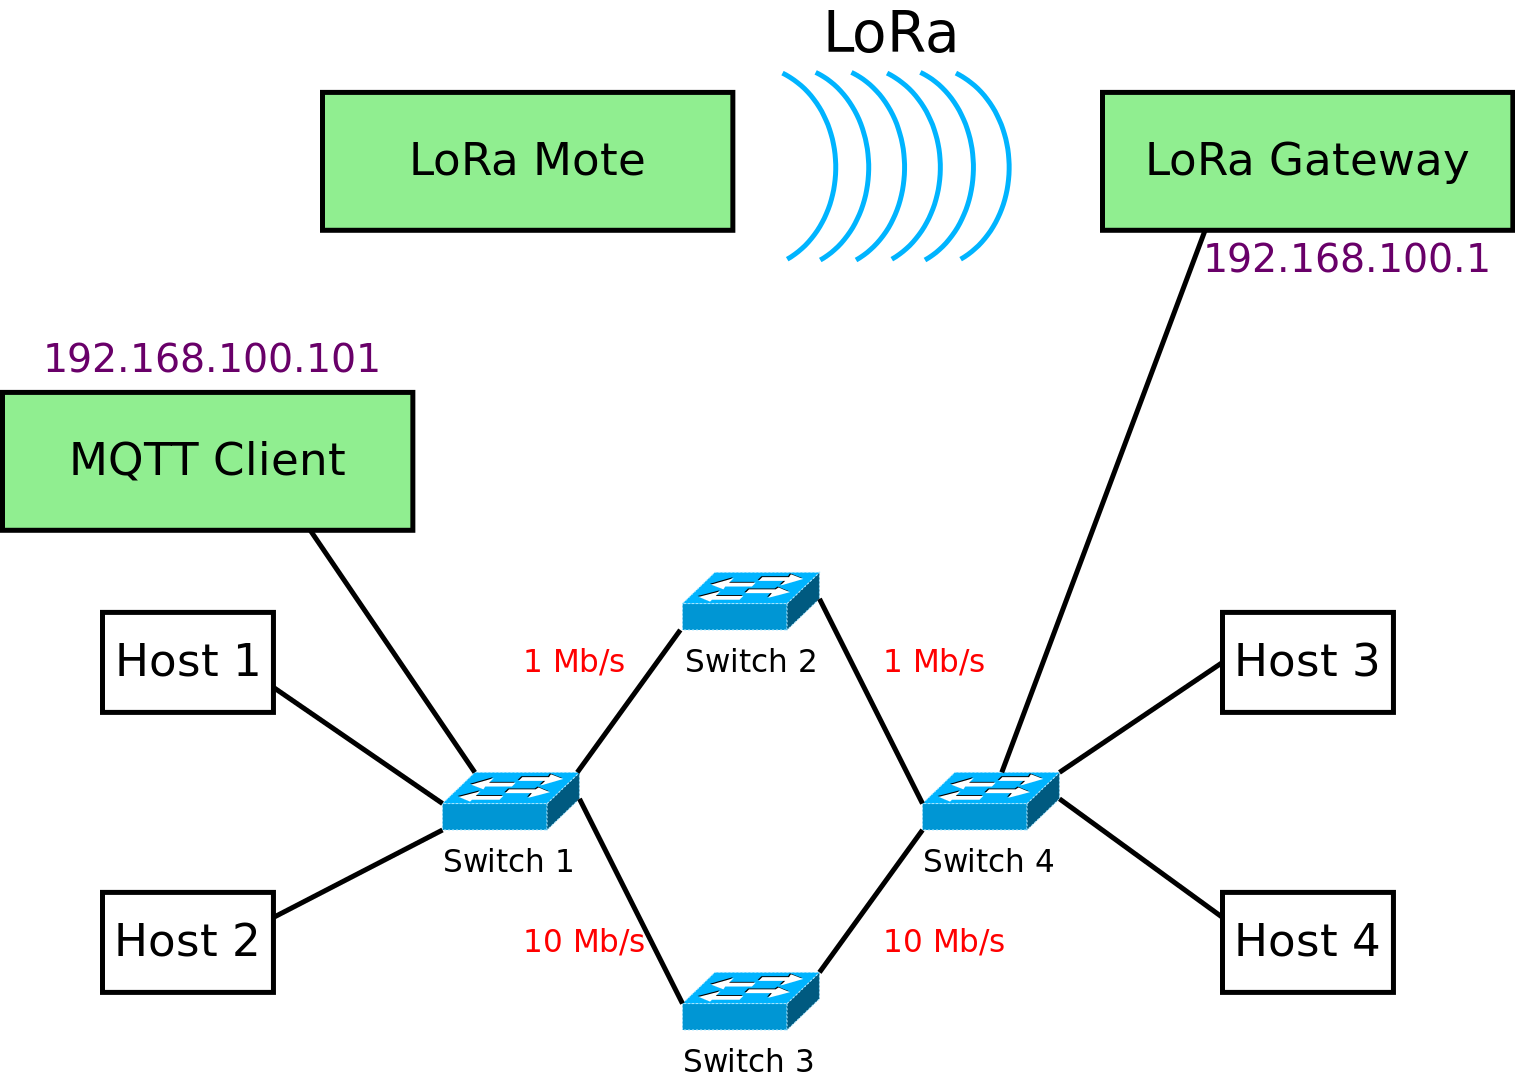
\includegraphics[width=\linewidth]{imagenes/Testing/mininet_topology_LoRa.png}
  \caption{Testing scenario for IP address slicing.}
  \label{fig:topology_LoRa}
\end{figure}

As for the MQTT client, we will use \textit{Mosquitto}.
\begin{lstlisting}
    mosquitto_sub -h localhost -t "gateway/#" -v 
\end{lstlisting}

Where:
\begin{itemize}
    \item \textbf{localhost}. Host where the messages are stored.
    \item \textbf{gateway/\#}. Topic we wish to subscribe to.
\end{itemize}

In addition, due to using Mininet within a virtual machine, the MQTT client must go through the physical Ethernet interface of the Mininet network host, which is not possible if said Ethernet interface does not belong to the same subnet, i.e., 192.168.0.0/16. There are several ways to accomplish this. We have opted to edit the configuration file at \textit{/etc/dhcpcd.conf}, adding the following lines at the end of the file:
\begin{lstlisting}
    interface eno1
    static ip_address=192.168.100.50/16
\end{lstlisting}

Where:
\begin{itemize}
    \item \textbf{eno1}. Name of our Ethernet interface on the Mininet network host.
    \item \textbf{192.168.100.50/16}. IP assigned to the interface. It can be any valid IP within the subnet as long as it is not already taken.
\end{itemize}

Lastly, for the test to be considered successful, every LoRa packet must be received at the MQTT client and packets must go through the slow path. To verify that this is the case, we will use the tool \textit{Tshark}, which is a terminal based packet sniffer.

\begin{figure}
  \centering
  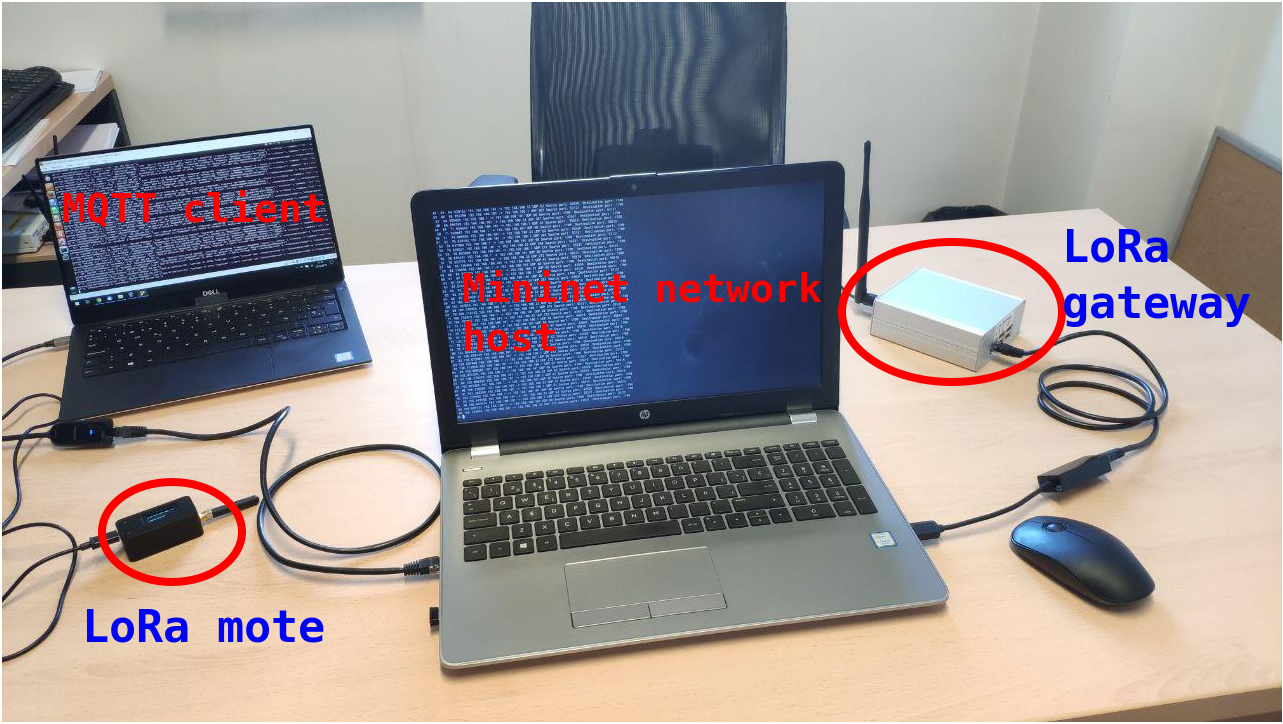
\includegraphics[width=\linewidth]{imagenes/Testing/lora_setup.png}
  \caption{Setup of the physical test components.}
  \label{fig:LoRa_setup}
\end{figure}

\subsection{Analysis of the Results}
Judging by Figure \ref{fig:mosquitto}, it looks like everything is working as expected. The LoRa packages are being forwarded correctly by the LoRa gateway and arriving at the MQTT client. Nevertheless, we still need to ensure that they are taking the correct path, as that is the actual point of this test. Thankfully, Figure \ref{fig:LoRa_tshark} shows that the packets are going through switch 2, which is the correct path, so everything is working correctly.

\begin{figure}
  \centering
  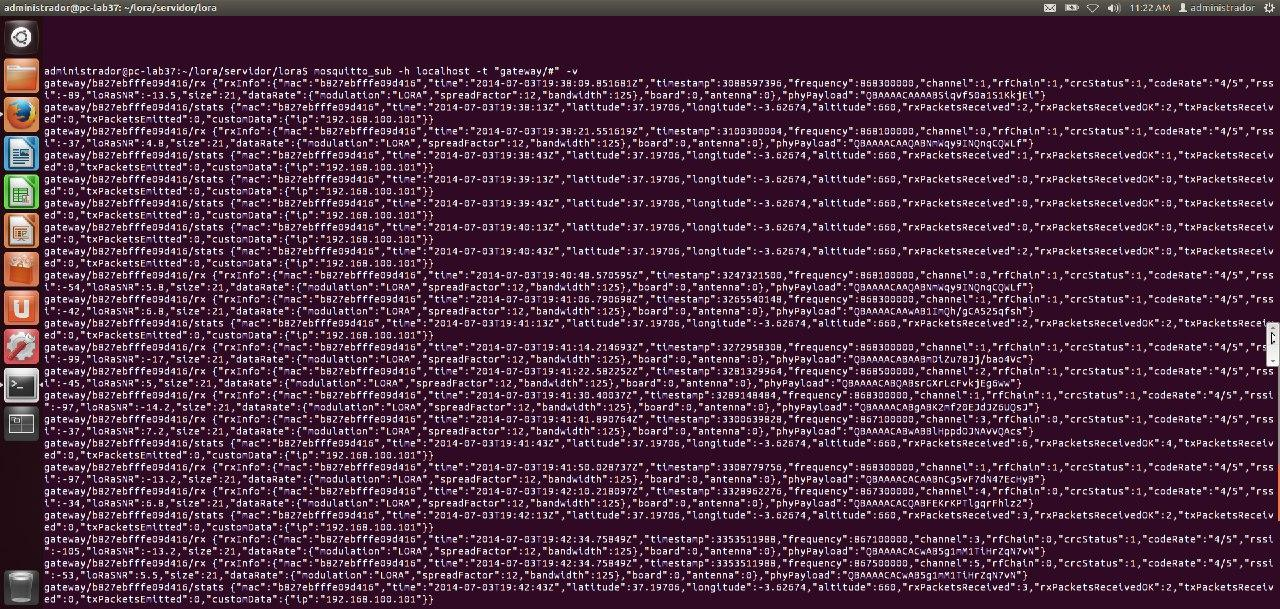
\includegraphics[width=\linewidth]{imagenes/Testing/mosquitto_packets.png}
  \caption{Packets shown on the MQTT client.}
  \label{fig:mosquitto}
\end{figure}

\begin{figure}
  \centering
  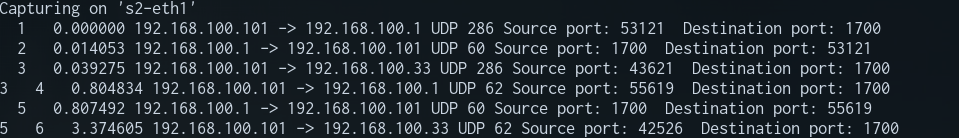
\includegraphics[width=\linewidth]{imagenes/Testing/tshark-LoRa.png}
  \caption{Packets sniffed by Tshark on switch 2.}
  \label{fig:LoRa_tshark}
\end{figure}

\cjorge{No recuerdo si has comentado que LoRaWAN se usa para IoT... haz algún comentario en este sentido, porque el lector puede no conocer LoRaWAN previamente.}

In this particular case, the slices help us isolate IoT traffic and send it through a slower path of the network. This way, we leave the faster path available for other types of traffic that require a higher bandwidth.

But, if we look past our example, there are many other ways in which it could benefit a real production network: providing traffic engineering for QoS, isolating traffic between different services or enabling a production network to be used as testbed for a different service among others possibilities. All in all, there is definitely a plethora of use-cases. 